% Program Studi D-IV Komputasi Statistik
% Politeknik Statistika STIS

\documentclass[conference, a4paper]{IEEEtran_ID}
\IEEEoverridecommandlockouts
\usepackage{cite}
\usepackage{fancyhdr}
\usepackage{lastpage}
\usepackage{amsmath,amssymb,amsfonts}
\usepackage{algorithmic}
\usepackage{graphicx}
\usepackage{textcomp}
\usepackage{xcolor}
\def\BibTeX{{\rm B\kern-.05em{\sc i\kern-.025em b}\kern-.08em
    T\kern-.1667em\lower.7ex\hbox{E}\kern-.125emX}}

\pagestyle{fancy}
\fancyhf{}
\lhead{}
\rhead{\footnotesize{Xinmiao Yu 518021910792}}
\lfoot{}
\rfoot{\thepage { /} \pageref{LastPage}}
\renewcommand{\headrulewidth}{0pt}
\renewcommand{\footrulewidth}{0pt}


\begin{document}

% Elemen judul proposal
\title{Kubernetes \\ 
\LARGE{A Container Management Platform} % Elemen subjudul proposal
}

\maketitle
\thispagestyle{fancy}

\section{Introduction}

The ubiquity of wireless networks and increasing number of electronic devices promote development of Internet of Things (IoTs), which highlights the high cost and difficulty of application deployment. Unlike the traditional deployment way such that run applications on a physical server directly, the container concept is introduced. It has some similarity of using virtual memory to address the memory limitation and program conflict problems. The containers behaved like virtual machines, but it is more lightweight. It is isolated from the underlying infrastructure so it is portable to deploy through cloud. 

\textit{Kubernetes} is an open-source platform used to bundle and run the applications in a production environment \cite{kudoc}. As IaaS (Infrastructure as a Service), PaaS(Platform as a Service) and SaaS (Software as a Service) are often used with cloud, \textit{Kubernetes} served a bit like Paas, with offering deployment, scaling, load balancing and etc\cite{ar1}.

\section{Basic Architecture} 
First to understand its mechanism, start with its architecture\cite{43826}.
	\begin{figure}[htbp]
		\centerline{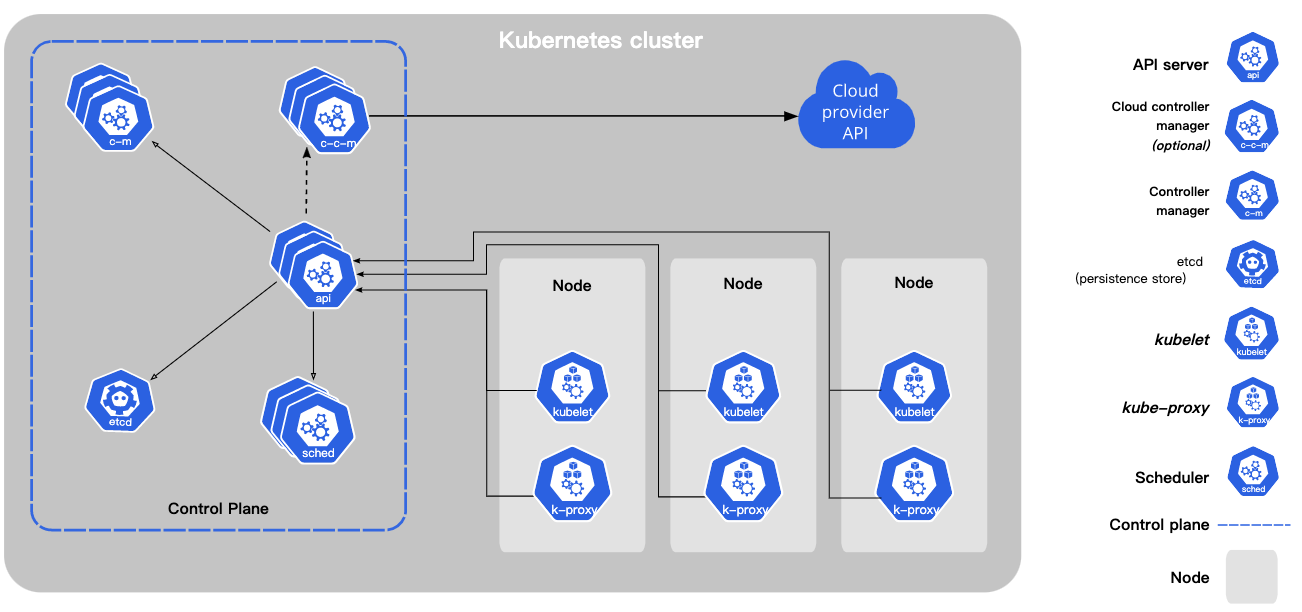
\includegraphics[width=0.5\textwidth]{kube.png}}
		\caption{Kubernetes Cluster\cite{kucom}}
		\label{dash}
	\end{figure}
\begin{itemize}
    \item A Kubernetes cluster consists of a master and various nodes, the control plane could be considered as utilized through the master.
    \item API server is used as the system's external interface, such that the control plane ``communicates" with the nodes through API server. Other components could call from it. 
    \item Scheduler is the whole system's scheduling part. As a cluster, there would exist problem for control plane such that which node to call, in which node deploy new application (contained by a pod).
    \item Controller manager is used to control the controller, including node controller, replication controller, endpoint controller, service account and token controller.
    \item ETCD is used to store the whole cluster's status. 
    \item Cloud controller manager and cloud provider API is used for cloud management and could be omiited. 
    \item Kubelet watch on each pod sent to its node, including pod creation, modification and deletion. 
    \item K-proxy is used to offer proxy for the node. The network communication within cluster is different, such that there will be virtual IP address for master to communicate with nodes and among different nodes. Calico and Flannel are popular network communication methods for Kubernetes cluster.  
    \item Pod is the atomic unit for deployment. Each time the apllication could be contained by a pod and deployed on one or more specific nodes, controlled by scheduler. Each pod could have various containerized app and some shared-resources for these containers, such as the shared storage, as volume. The IP address of this pod, called Pod IP address, is used for all containers with this pod. The pod will also store the information of how to run each container so the node could utilize the containers within the pod. 
    \item Service is used to combine many pods, and a service in whole could be used. DNS could be used to address the problem that the services visiting each other, through the service name to visit the virtual IP address. And for user, ingress is used to visit on master.
    
\end{itemize}
\section{Special Properties}
\textit{Kubernetes} is already widely used in industry. For example, Ant Financial has huge scale of data processing, it is really  challenging to do real-time compute, storage, and processing capability as well as ensure the security \cite{ant}. They begun to use containers in 2014, and migrated the production workload to the \textit{Kubernetes} platform. There are some special properties that might cause \textit{Kubernetes} to be so popular. 
\begin{itemize}
    \item DaemonSet. It could be configured for different pods. The when a new node join in the cluster, this pod with DaemonSet could be automatically deployed on the new node. When a node is deleted from the cluster, the pod will be safely deleted as well\cite{kudeamon}. We could see the efficicency of the cluster with such mechanism, as in industry a huge cluster is highly likely to be used. An automatically set up and deletion is very useful.
    \item ReplicaSet. It is used to ensure at each time, the number of pods running is a certain fixed number. So even when a node is shuttled down accidently, the service provided will not be influenced. 
    \item Deployment. It could realize the function of replicaset but with more properties. Or it is same to view replicaset is implemented through Deployment. The pod could be deployed through the deployment. It provides a simple way to manage resources. New deployment could have all the resources from an old deployment. 
    \item Customization. The \textit{Kubernetes} cluster could be customized through changing scheduler, which default is Kube-Scheduler. It is commonly appeared in Federated Learning areas. Because for Federated Learning, its critical difference with Machine Learning is how the resources or models are allocated to different clients  (nodes). So the default scheduler of \textit{Kubernetes} could be replaced by a special customized scheduler using configuration file\cite{8486422}. This might be more useful for research areas.
\end{itemize}


\section{Potential Limitations}
Although it is widely used in industry, it still exists some limitations. As a new and developing open-source platform, it's still upgrading and developing new features. Because we do not need to do much coding for building such a platform, it is highly correlated to potential issues during running. Although suggested in \cite{8486422} that \textit{Kubernetes} could be used for Machine Learning, there might be some problems even though \textit{Kubernetes} has install instruction and quick setup.
\begin{itemize}
    \item Version. Because of the continuous upgrading, various version might support different devices, and the components version is specified for one specific version.
    \item Inconsistent default setting. Different components for \textit{Kubernetes} have inconsistent settings, and the modification of the default setting might fail. So the customization might not be well supported.
    \item Communication within cluster. As introduced before, it uses different network communication method. It needs to be decided before the initialization, but due to the real world devices limit, the network policy, or the container network plugin might be changed.
    \item Various standard.  The Raspheery Pi could not join the cluster, although the official documents claim the support for Raspherry Pi. Because if installed the GUI, it will not be supported anymore. 
\end{itemize}

The troubleshooting for \textit{Kubernetes} is not so understandable and the solutions often needs a long time searching as well as reading the logs. But the varying situation make it difficult to find the right solution. Integrated with a problem diagnosis using log might be a future developing direction \cite{8119164}. A precise log model is provided and the experimental results show their approach can find out the real-world \textit{Kubernetes} problems. So the potential development might be a lower application threshold, as for now, one corporation might still need advanced engineers to apply and maintain this system, which limits a more extensive usage. 

\bibliographystyle{IEEEtran}
\bibliography{Proposal}

\end{document}
